\documentclass[12pt]{report}
\usepackage{setspace}
\usepackage{amsmath,amssymb}
\usepackage{amsfonts}
\usepackage{todonotes}
\usepackage{graphicx}
\usepackage[pdftex,bookmarks=true,bookmarksopen=false,bookmarksnumbered=true,colorlinks=true,linkcolor=black]{hyperref}
\usepackage{float}
\usepackage[utf8]{inputenc}
\usepackage{natbib}

\begin{document}

\begin{titlepage}
\begin{center}
{\LARGE Getulio Vargas Foundation}\\
\vspace{0.3cm}
{\LARGE Applied Mathematics School}\\
\vspace{0.3cm}

\par
\vspace{170pt}
  \textbf{\Large {Machine learning aproach for Dengue forecasting - Comparing LSTM, Random Forest and Lasso}}\\
  
\vspace{32pt}
{\Large Elisa Mussumeci}\\
\end{center}

\par
\vfill
\begin{center}
{{\normalsize Rio de Janeiro}\\
{\normalsize \the\year}}
\end{center}
\end{titlepage}

\thispagestyle{empty}

\newpage
\begin{center}
\textbf{\LARGE Elisa Mussumeci}

\par
\vspace{200pt}
\textbf{\Large Machine learning aproach for Dengue forecasting - Comparing LSTM, Random Forest and Lasso}
\end{center}

\par
\vspace{85pt}
\hspace*{175pt}\parbox{7.6cm}{{\normalsize Dissertação submetida à Escola de Matemática Aplicada como requisito parcial para a obtenção do grau de Mestre em Modelagem Matemática da Informação.}}

\par
\vspace{1em}
\hspace*{125pt}\parbox{10.0cm}{{\normalsize Área de Concentração: }}

\par
\vspace{1em}
\hspace*{125pt}\parbox{10.0cm}{{\normalsize Orientador: Flávio Codeço Coelho}}\\

\par
\vfill
\begin{center}
{{\normalsize Rio de Janeiro}\\
{\normalsize \the\year}}
\end{center}

\thispagestyle{empty}

\newpage
\noindent{\textbf{\large Acknowledgements}}\\
\doublespacing
Gostaria de agradecer....

\thispagestyle{empty}

\newpage
\begin{center}
\textbf{\normalsize Resumo}
\end{center}
\vspace{1pt}

resumo...

\thispagestyle{empty}

\newpage
\begin{center}
\textbf{\normalsize Abstract}
\end{center}
\vspace{1pt}

We use the Infodengue database of incidence and climate time-series, to train predictive models for the weekly number of cases of dengue in 733 cities of Brazil. To overcome limitation in the length of timeseries available to train the model, we included the time series of similar cities as predictors in the model of each city. The LSTM recurrent neural network model attained the highest performance in predicting future incidence on dengue in cities of different sizes. 

\thispagestyle{empty}

\newpage
\tableofcontents
\listoffigures
\thispagestyle{empty}

\newpage
\chapter{Introduction}


The quick spread of diseases like Dengue, Zika and Chikungunya impacts the health, social, and economies of many countries around the world. That makes prediction models for epidemiological time series very relevant, since it can help the health authorities and the population to prepare for a potential epidemic \citep{luz2008time}. 


Understanding and therefore being able to predict the incidence of vector-borne diseases is a big challenge due in part to the complex interplay between epidemiological and environmental determinants but also due to the frequent lack of long-term records of historical disease incidence and other cofactors affecting risk. This complex dynamics manifests itself in the variability of the of th incidence patterns in different geographical areas[ref].

In the case of dengue, the effects of climate of the vector's population dynamics impose a marked seasonality which is then modulated by variations in the immunologica structure of the population as well as by human demography[ref].

Modeling dengue incidence patterns in Brazil presents an aditional challenge characterized by the fact that the disease was reintroduced in the country in the 1980s having been absent for many decades. Therefore, basides the problem of short time series we are dealing with a disease which has yet to reach its endemic equilibrium. Any forecasting model hoping to grasp the complex temporal dynamics of dengue will require a large amount of data.

In this paper, we use the Infodengue[ref] database of more than 700 cities in Brasil since 2010. To make up for the relatively short timeseries, we use use incidence series from epidemiologically similar cities as predictors, together with relevant environmental timeseries for each city to fit predictive models capable of forecasting the weekly incidence of Dengue for any city of Brazil across a wide range of latitudes and climate characteristics.

Instead of proposing parsimonious models built from previous knowledge of the determinants of dengue transmission, we fit machine learning models known for their ability to navigate their way into data intensive high dimensional problems, by integrating variable selection into their fitting routine. Namely we will compare the following models: LSTM, a recurrent deep neural network model[ref], Random Forest regression and LASSO regression[refs].

\newpage
\chapter{Literature Review}

\section{Time Series}
\subsection{Multiple time series regression}


\section{Epidemic forecasting}
 
Time series forecasting consists in use models to predict future values based on previously observed values.
 
 
In epidemiology studies, forecasting is important to understand disease spread over a period of time

It's commom to use time series forecasting models to predict epidemic
 
The most comon models used for epidemic forecasting are:
 
 \begin{description}
  \item Autoregressive Integrated Moving Average (ARIMA)
  \item Seasonal Autoregressive Integrated Moving Average (SARIMA)
  \item VAR
 \end{description}

Apresentar a diferença entre predição de series temporas simples e multiplas. Explicar cada modelo que vem sendo utilizado em prediçao multipla


\section{Hierarchical Clustering}
\subsection{clustering time series}

\section{Machine Learning and forecasting}

machine learning is bla bla

machine learning techniques have been used to forecast as show in ref and ref. It bring good results since
it cand bla bla ref.

Neural networks is one technique that has been researched quite 
extensively, and has often been shown to beat time series approaches ref 

explain why these kind of models are good for forecasting

\subsection{Random Forest and Lasso}

\begin{description}
 \item Random Forest
  
 Random forests  are an ensemble learning method for classification, 
 regression and other tasks, that operate by constructing a multitude of decision trees at training time 
 and outputting the class that is the mode of the classes (classification) or mean prediction (regression) 
 of the individual trees.
 
 Decision tree learning is a method commonly used in data mining. The goal is to create a model 
 that predicts the value of a target variable based on several input variables. 
 
 The difference between Random Forest algorithm and the decision tree algorithm is that in 
 Random Forest, the process es of finding the root node and splitting the feature nodes will run
 randomly.
 
 Add formula
 
 \item Lasso
 
 In statistics and machine learning, lasso (least absolute shrinkage and selection operator)
 (also Lasso or LASSO) is a regression analysis method that performs both variable selection and
 regularization in order to enhance the prediction accuracy and interpretability of the statistical
 model it produces. It was introduced by Robert Tibshirani in 1996 based on Leo Breiman’s
 nonnegative garrote.
 
 Lasso was originally introduced in the context of least squares, and it can be instructive to consider 
 this case first, since it illustrates many of lasso’s properties in a straightforward setting.
 
\end{description}


\subsection{Long-short term memory (LSTM)}

Recurrent neural networks ADD REF are neural networks with loops in them, allowing information
to persist. They can be thought of as multiple copies of the same network, each passing a message
to a successor.

RNN's have great performance  in most cases but they can't handle long-term dependencies. That 
means that when the gap between the relevant information and the output is too large, the network
become unable to learn to connect the information.

Long Short Term Memory networks (add ref )are a special kind of RNN, capable of learning
such long-term dependencies. In each cell of chain the network decides whoch informations to keep
and which to forget, etcs

add colah diagram step by step

\newpage
\chapter{Article}

\section{Methodology}


\subsection{Data sources}
The dataset used in the article was provided by the InfoDengue project. 

InfoDengue \citep{Codeco046193} is an integrated dengue alert system, developed as a partnership between Oswaldo Cruz Foundation, Getulio Vargas Foundation and the Ministry of health. As a unique source of carefully curated data for epidemiological studies, InfoDengue monitors 604 cities in Brazil, predicting the weekly number of new cases of dengue in each one of them.

The data consist of the weekly series of dengue incidence,  temperature, humidity, pressure, precipitation intensity, and tweets about Dengue in each observed city. It ranges from 2010 until today.

\begin{figure}
 \centering
 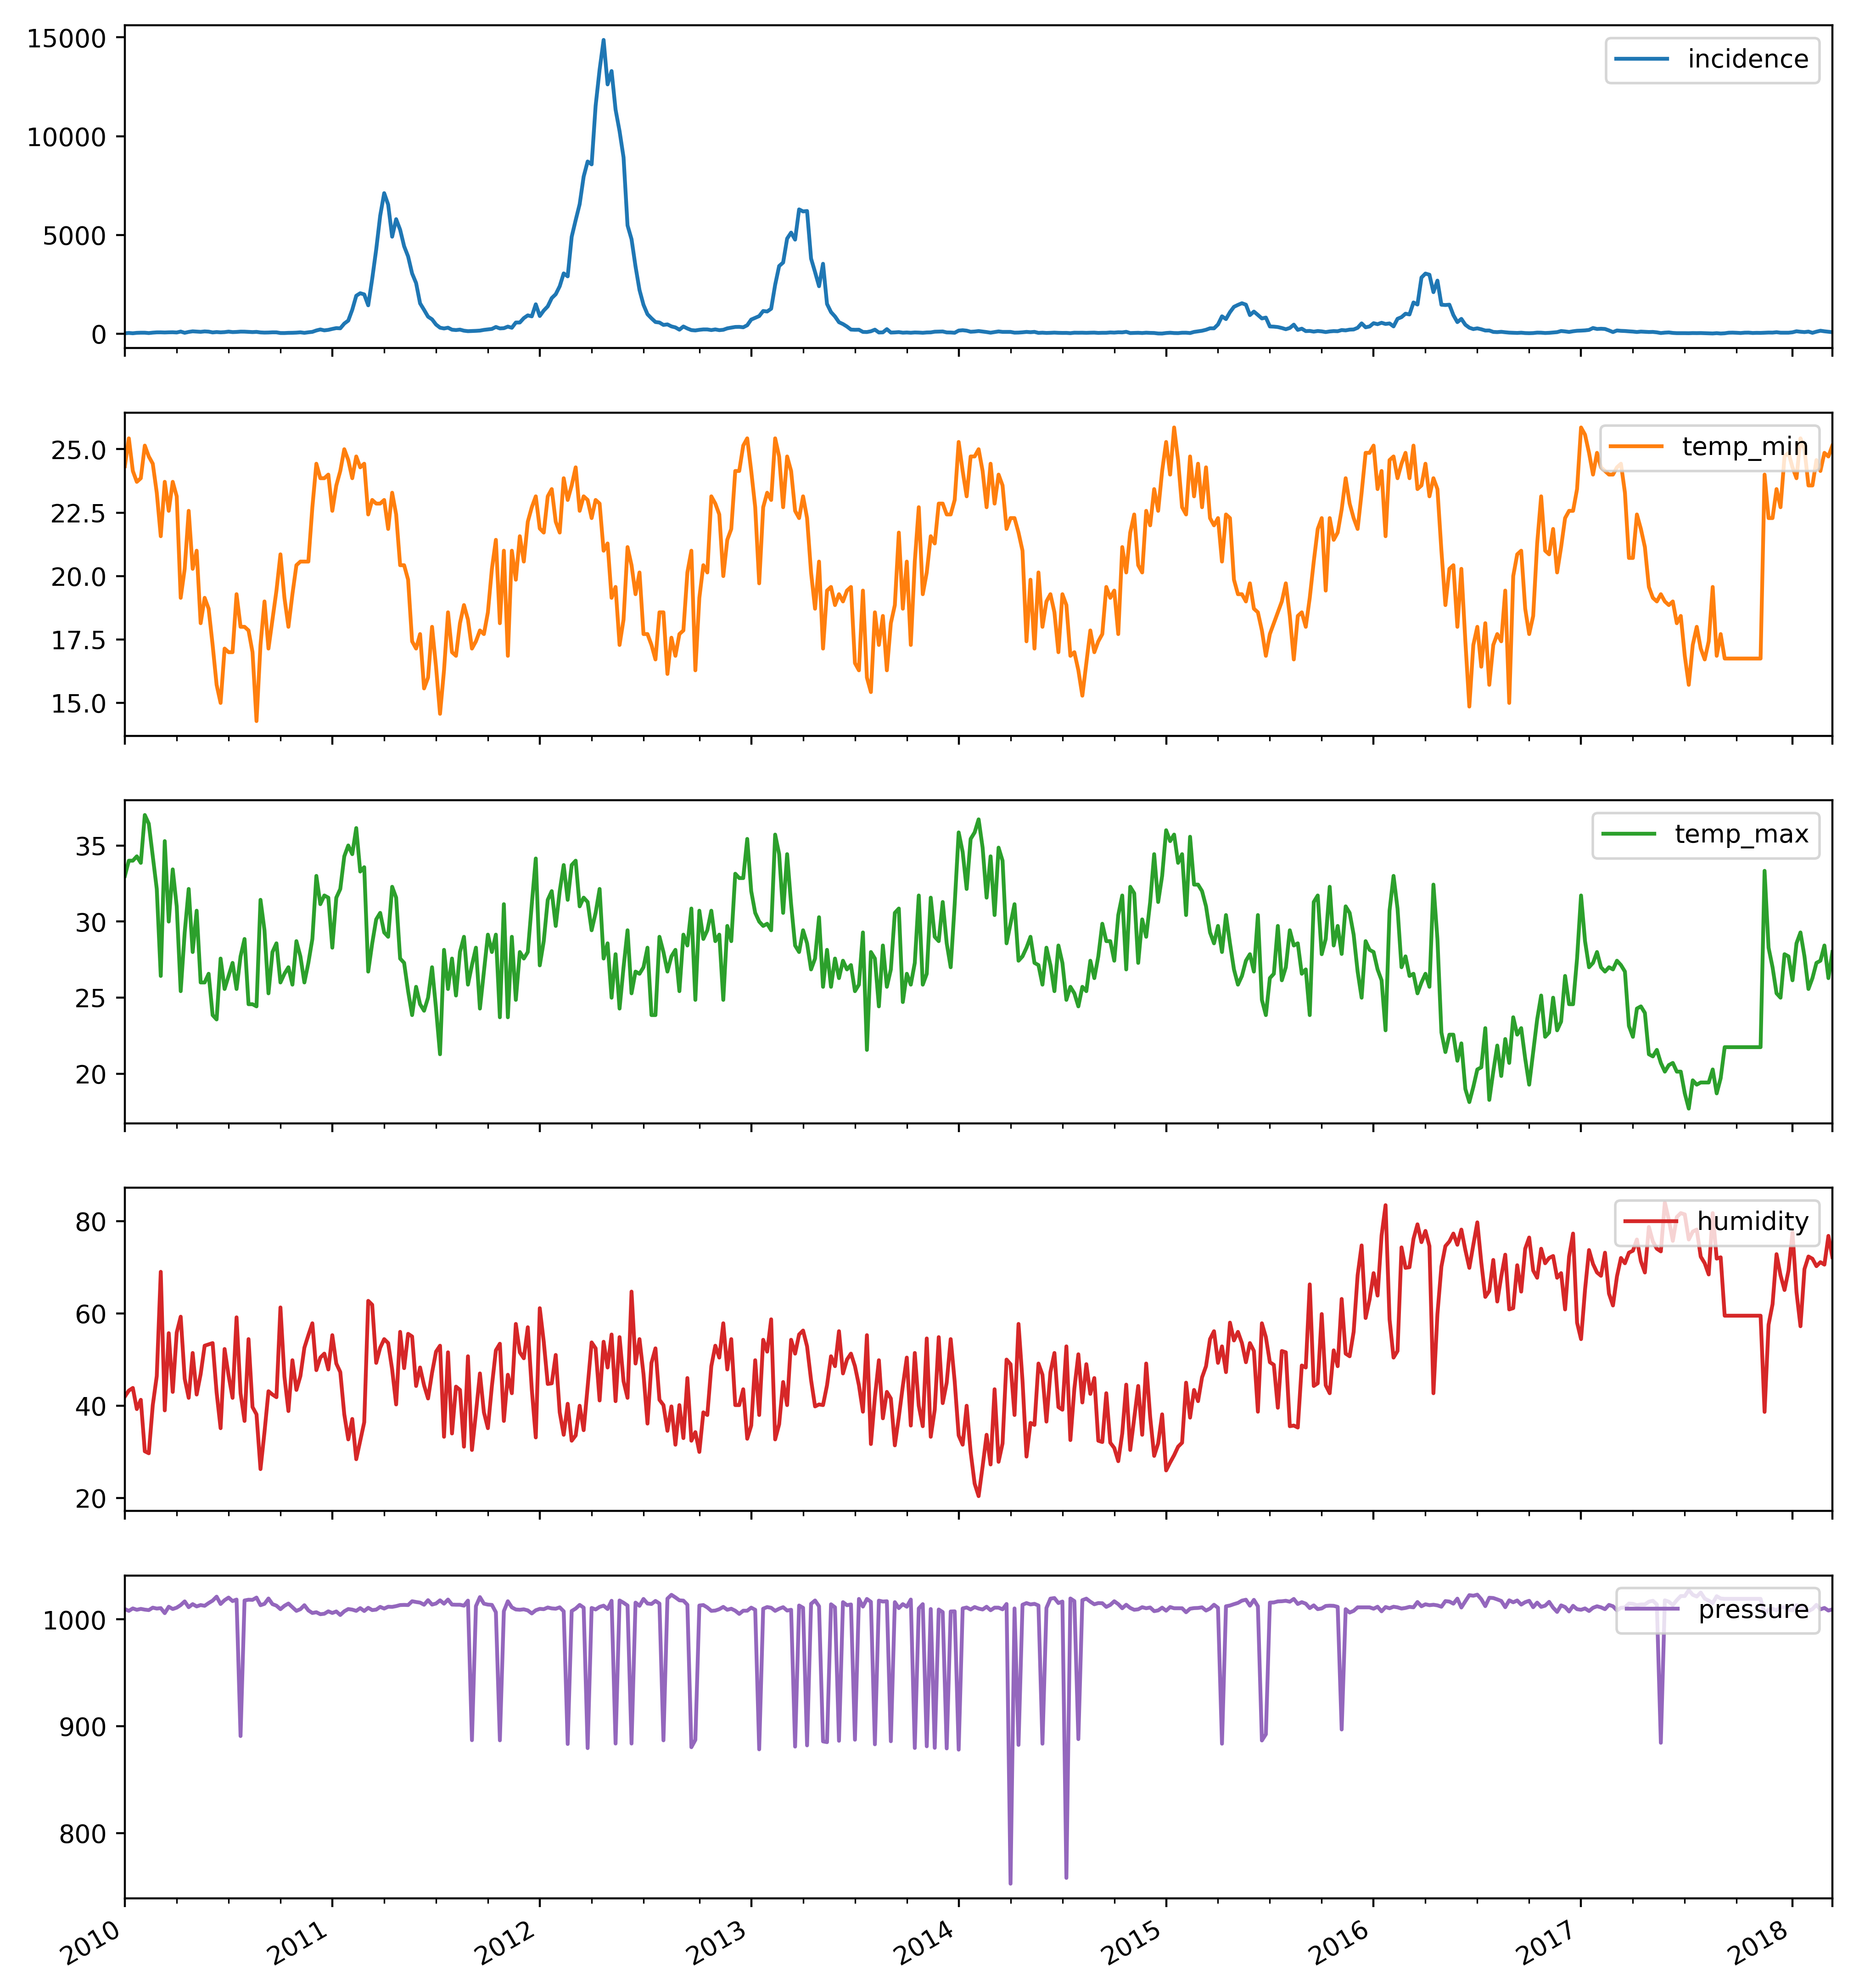
\includegraphics[width=\textwidth]{rio_raw_series.png}
 % rio_raw_series.png: 4000x4000 px, 400dpi, 25.40x25.40 cm, bb=0 0 720 720
 \caption{Time series from Rio de Janeiro features}
 \label{fig: rio_raw}
\end{figure}

\todo[inline]{as séries têm que começar em 2010, mesmo que os tweets só comecem em 2012}

\subsection{Data modeling}

It is very difficult to accurately forecast the weekly incidence in a city based only on its historical data. This happens mainly because of the spatial component of disease transmission. Diseases perpetuate themselves by moving from population to population. The flow of individuals between cities is also an important factor.

Dengue is a disease with a clear spatial dependency \citep{stoddard2013house,eisen2009use}. Therefore it makes sense to uses series from neighboring cities nearby in order to reduce uncertainty. Additionally, other cities not necessarily in the vicinity but which display similar historical series of incidence, can also be included as predictors.

In order to define the set of cities with relevant predictive information for each city, we clustered all cities within a state based on the correlation distances between incidence time series for each pair of cities. The clusters were calculated hierarchically, where the distance $d$ of each pair of clusters $(u,v)$ was given by the Farthest Point Algorithm:

$$d(u,v) = max(dist(u[i],v[j])), $$

for all points $i$ in cluster $u$ and $j$ in cluster $v$. The threshold is set to $0.6*max(z))$, where $z$ is the vector of the pairwise correlation distances of the cities. We can see in  \ref{fig:corr_rj} the correlation matrix of the cities from the state of Rio de Janeiro, the treshold define the distance between the clusters in \ref{fig:cluster_rj}.

\begin{figure}
 \centering
 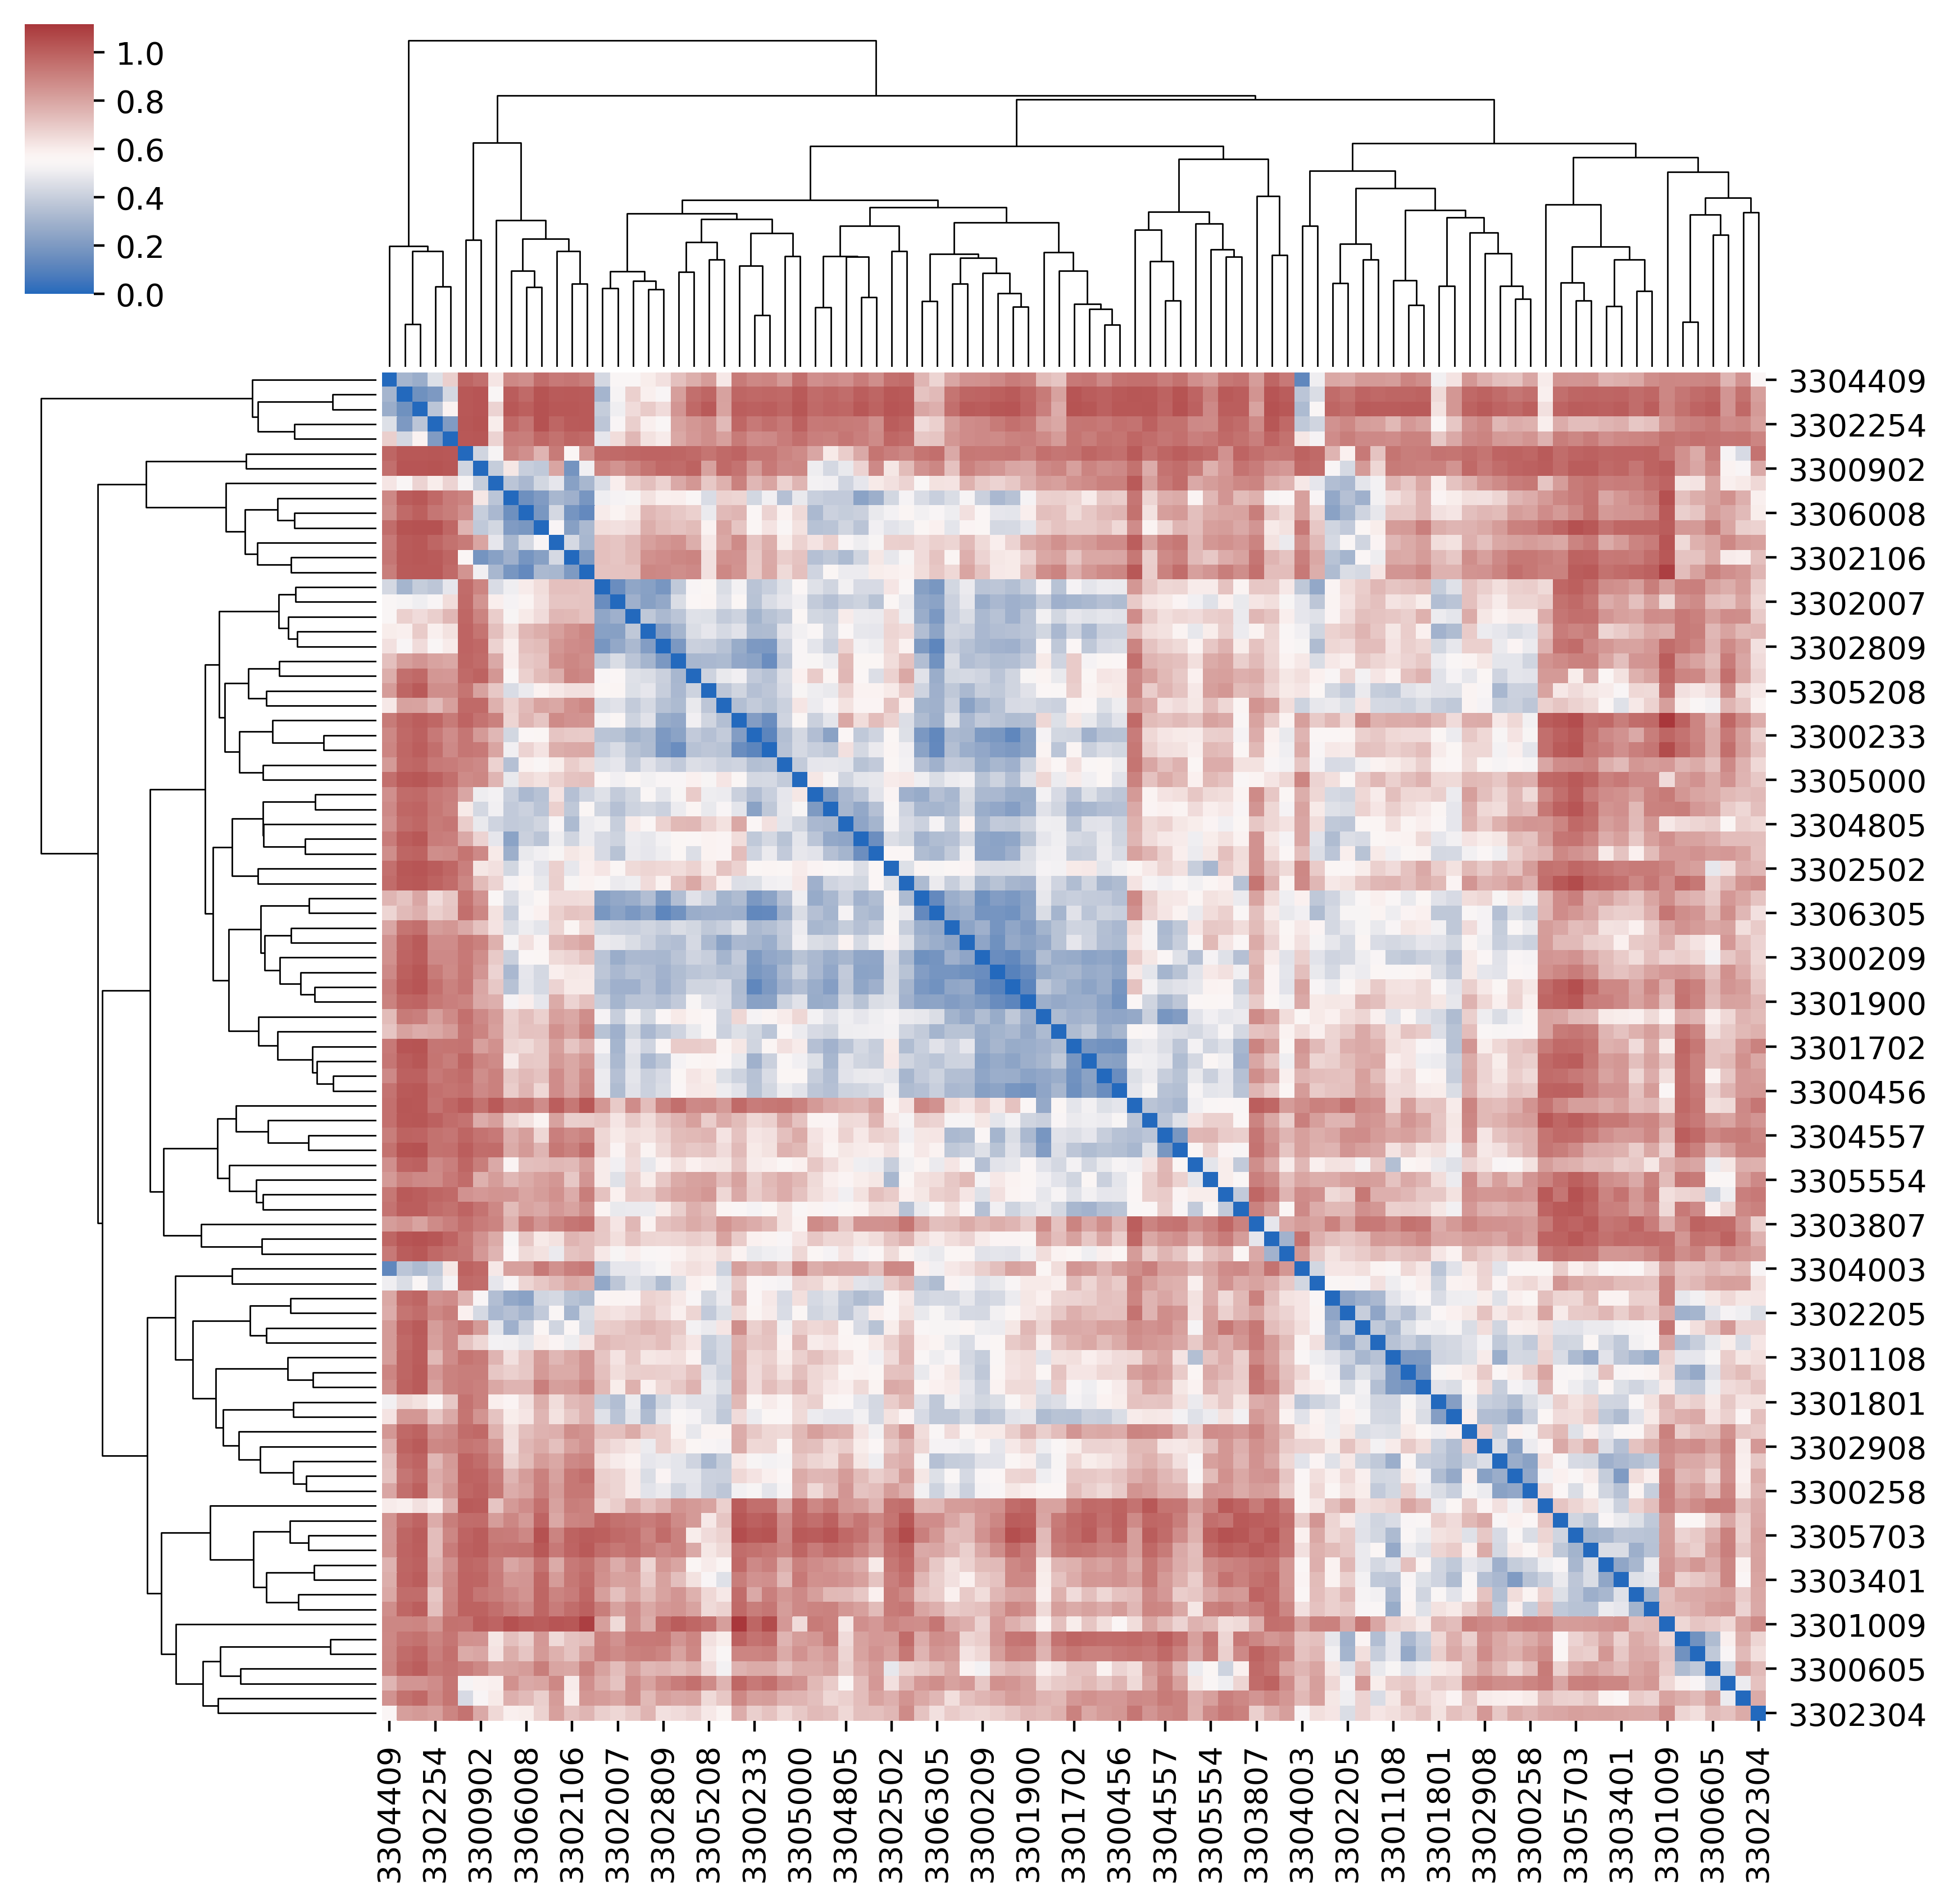
\includegraphics[scale=0.4]{cluster_corr_RJ.png}
 % cluster_corr_RJ.png: 3469x3389 px, 400dpi, 22.03x21.52 cm, bb=0 0 624 610
 \caption{Distance matrix of cities for the state of Rio de Janeiro.}
 \label{fig:corr_rj}
\end{figure}


\begin{figure}
 \centering
 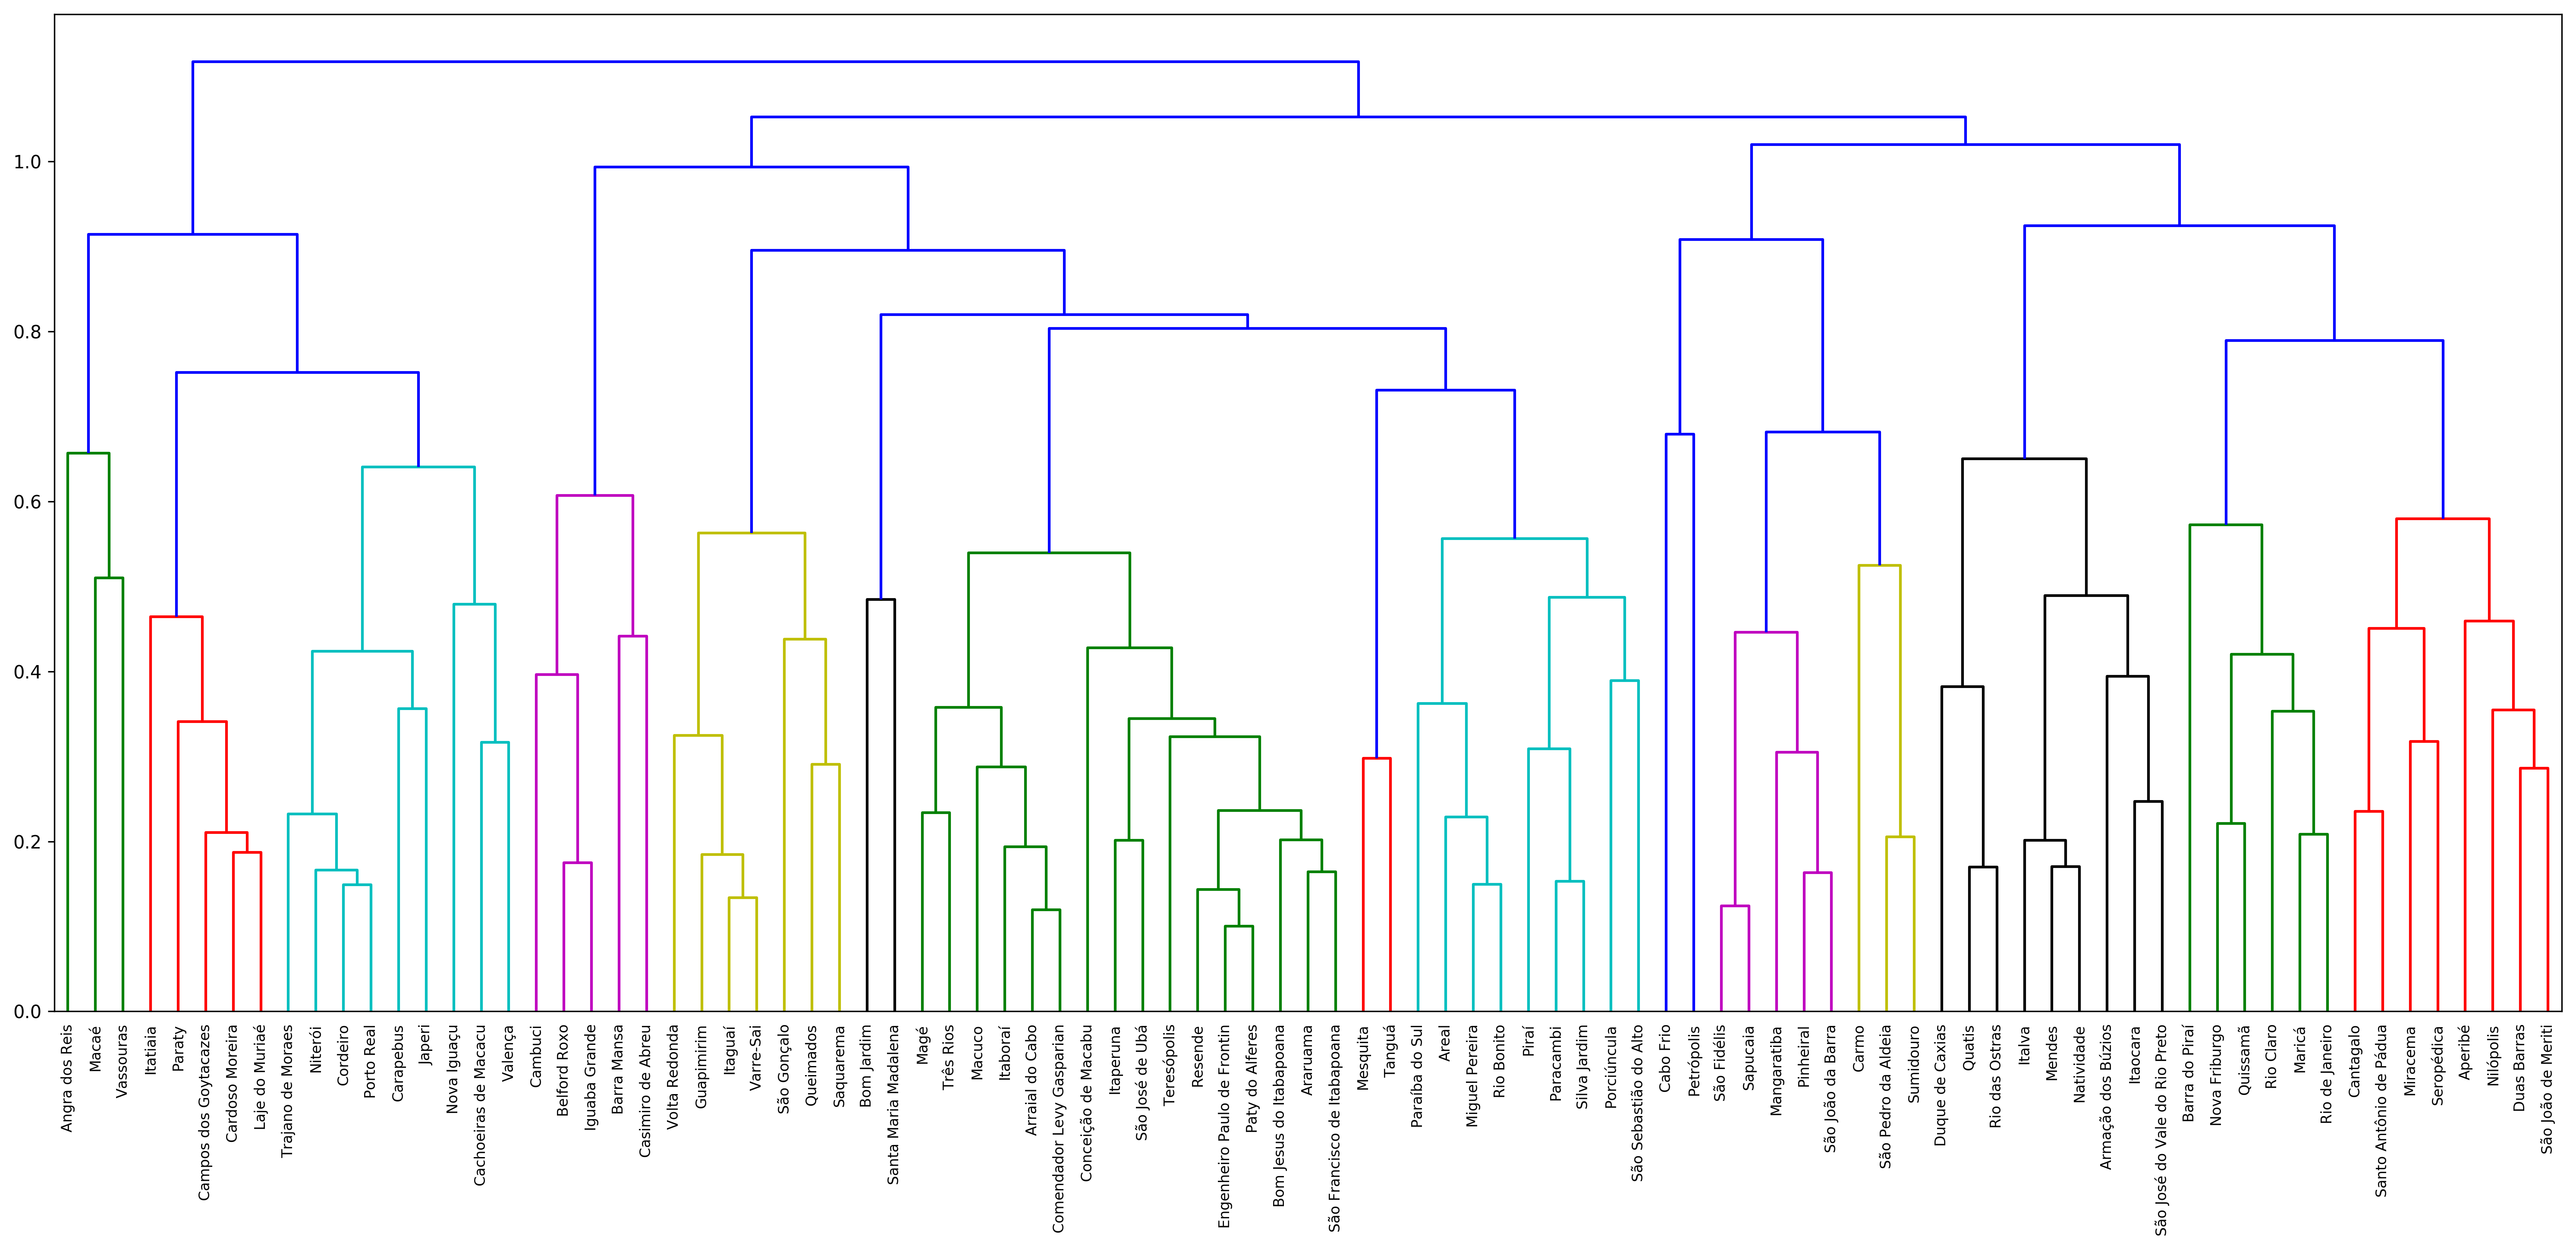
\includegraphics[width=\textwidth]{clusterRJ_06.png}
 % clusterRJ_0.6.png: 5971x2894 px, 300dpi, 50.55x24.50 cm, bb=0 0 1433 695
 \caption{Hierarchical cluster of Rio de Janeiro.}
 \label{fig:cluster_rj}
\end{figure}

For each city, a feature matrix was assembled from the set of time series of 
each other time series from its cluster.
\todo[inline]{matrix example of the data clustered - Coloco uma generica ou um corte da real? Põe uma genérica indicando as features usadas}

A single city model was fitted  for a few  cities to serve as a 
baseline against which to compare the effectiveness of the using a cluster of  
cities as predictors.

\subsection{Forecasting}

We fit tree different classes of models to forecast the incidence timeseries. For all models we adopted a forecast window of 4 weeks, meaning that from any moment in time the model will generate forecasts for the next 4 weeks based only on historical data up to that point.

\begin{description}
 \item \textbf{Random Forest:}
 We used a Random Forest regression model to predict a single point in the future based on historical data. In order to turn a time series prediction problem into a regression model, we transformed the series regressors into a vector containing not just the last observation of each series but the {\cal D} most recent.
 
\begin{equation}
y_{D+\tau} = \sum_{d=0}^{D-1} \beta_d X_{t-d}
\end{equation}

$X_{t-d}$ is the vector with the values of all predictor series at time $t-d$, including $y$. The model predicts the incidence at a particular week in the future $y_{D+\tau}$, thus since we wanted to predict 4 weeks into the future, 4 separate models were fitted to data with $\tau$ varying from 1 to 4.


\begin{tabular}{cccc|c}
 $f_1$ & $f_2$ & $f_3$ & $f_4$ & $2$\\
 $f_2$  & $f_3$ & $f_4$ & $f_5$ & $1$\\
\end{tabular}

\todo[inline]{colocar aqui um exemplo da feature matrix $X$}

 
 \item \textbf{Long short term memory (LSTM)}
 A LSTM model is a recurrent deep neural network model developed to handle predictions of timeseries. We used a LSTM model with topology given in table xx. the model was trained for 300 epochs using a MLSE loss function defined in equation (xx) A look back 
of 4 weeks a forecasting window of 4 weeks was chosen.
\todo[inline]{descrever o tensor de dados do modelo LSTM}

 
 A LSTM model was defined with topology given in table xx. the model was trained 
for 300 epoch using a custom loss function defined in equation (xx) A look back 
of 4 weeks a forecasting window of 10 weeks were chosen.


 
 \item \textbf{Lasso regression:}
  A LASSO model is an estimator for linear regression models which also performs variable selection as it can estimate sparse coefficient matrices. We used the same feature matrix used by the Random Forest model for the LASSO model; Additionally, we applied an evolutionary tree-based optimization procedure proposed by \citet{Olson_Bartley_Urbanowicz_Moore_2016} to define the final LASSO model.
 
\end{description}


\section{Results}

\subsection{Cluster analysis}

We performed the clustering of cities as described above for every state in the Infodengue dataset. Figure \ref{fig: cluster_cf} shows the incidence series for one cluster for the entire historical period available. We can see that cities clustered together display similar incidence patterns. Depictions of the remaining clusters can be found in the supplementary material. Cluster sizes are variable.


The cluster found within each state are shown in figures ... The clusters can 
also be seen in the map in figures xxx.
\begin{figure}[h]
 \centering
 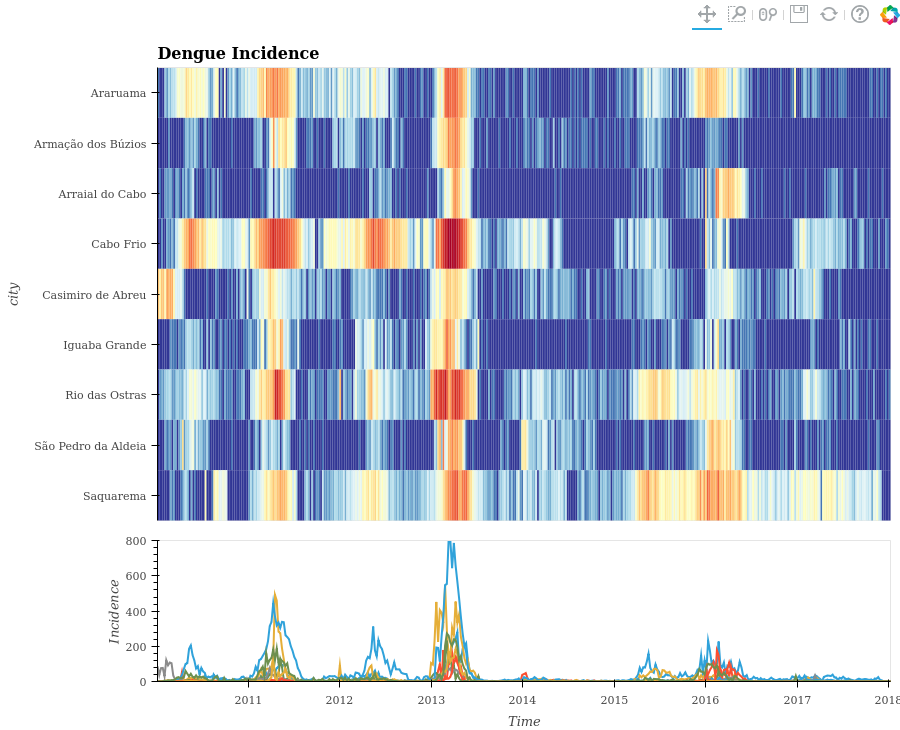
\includegraphics[scale=0.4]{./cluster_3300209.png}
 % cluster_3300209.png: 0x0 pixel, 300dpi, 0.00x0.00 cm, bb=
 \caption{cluster}
\end{figure}

\subsection{Forecasting}
We measured the performance of the forecasting models by the magnitude of the prediction error for week $t+4$ where $t$ is the last week observed. The prediction errors were calculated as mean squared error (MSE), and mean squared log error(MSLE).

Figures xx and yy show the performance of the prediction  both \emph{in-sample} 
and  \emph{out-of-sample}.

forecasting with cluster and without cluster?

\section{Discussion}

The model has show good performance for both large and small cities from various parts of Brasil. This shows that the set of predictor series selected is capable to characterize the epidemic dynamics.

The extra information provided by the sister cities' series alowed the model to substantially outperform the base model. The LSTM model was capable of consistently predict the incidence pattern of non-epidemic years. 

\newpage
\chapter{Conclusions and Final Considerations}

\newpage
\phantomsection
\addcontentsline{toc}{chapter}{References}
\bibliographystyle{model1-num-names}
\bibliography{sample}

\newpage
\phantomsection
\addcontentsline{toc}{chapter}{Appendices}

\end{document}
